\documentclass{beamer}
\usepackage{graphicx}
\usepackage{listings} % Syntax highlighing
\usepackage{fancyvrb} % Inline verbatim

\usetheme{Boadilla}
\title{PLACEHOLDERS}
\author{UMBC Malware Data Science}
\date{2020}

\begin{document}

\begin{frame}{Shannon's Entropy}
    \only<1>{$$ H=-\sum_{n=0}^{n-1}n_x\log_2 n_x $$}
    \only<2>{
        \begin{itemize}
            \item For our purposes, entropy is the measurement of randomness in a file.
            \item Entropy range is zero to 8.
            \item English text has an entropy of around 4.
            \item Typical machine instructions have an entropy of around 5.5 to 6.
            \item Encrypted or packed content has an entropy of 7.8 to 8.
        \end{itemize}
    }
    \only<3>{
        Entropy can be visualized as a histogram: \\ ~~ \\
        \begin{columns}
        \column{0.5\textwidth} {
            \small Entropy of 4.88
            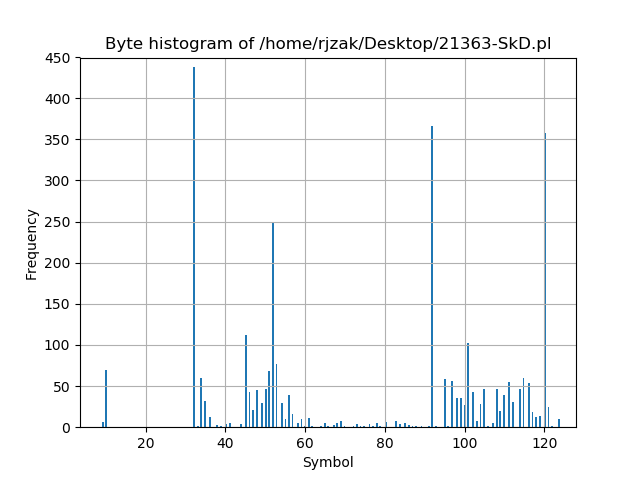
\includegraphics[width=6cm]{Images/Perl_script_histogram.png}
            }
        \column{0.5\textwidth} {
            \small Entropy of 7.96
            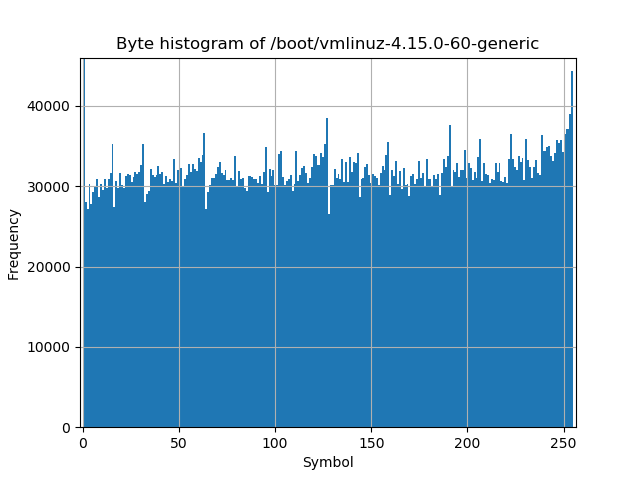
\includegraphics[width=6cm]{Images/Linux_Kernel_histogram.png}
            }
    \end{columns}
    }
\end{frame}

\end{document}